\documentclass[10pt,a4paper]{article}
\usepackage[latin1]{inputenc}
\usepackage{amsmath}
\usepackage{amsfonts}
\usepackage{amssymb}
\usepackage{fullpage}
\usepackage{graphicx}
\usepackage{parskip}

\begin{document}
\title{J.D. Jackson Problem 1.8}
\author{Josh Orndorff \\ admin@joshorndorff.com}
\maketitle

\section{Parallel Plates}
The electric fields of the two plates cancel each other outside of the capacitor, but add together inside for a total electric field in the region between the plates of
\begin{equation}
E=\frac{\sigma}{\epsilon_0}
\end{equation}

We can calculate the energy density between the plates according to equation 1.55 in the text. Of course the energy density is zero outside the plates.
\begin{equation}
w=\frac{\epsilon_0}{2}|\mathbf{E}|^2
\end{equation}

Now we just substitute the field from above. We can also use the relationship $\sigma=\frac{\epsilon_0 V}{d}$ from problem 1.6 to get energy density in term of electric potential between the conductors.
\begin{equation}
w=\frac{\sigma^2}{2\epsilon_0}=\frac{\epsilon_0 V^2}{2d^2}
\end{equation}

\begin{figure}[h]
\centering
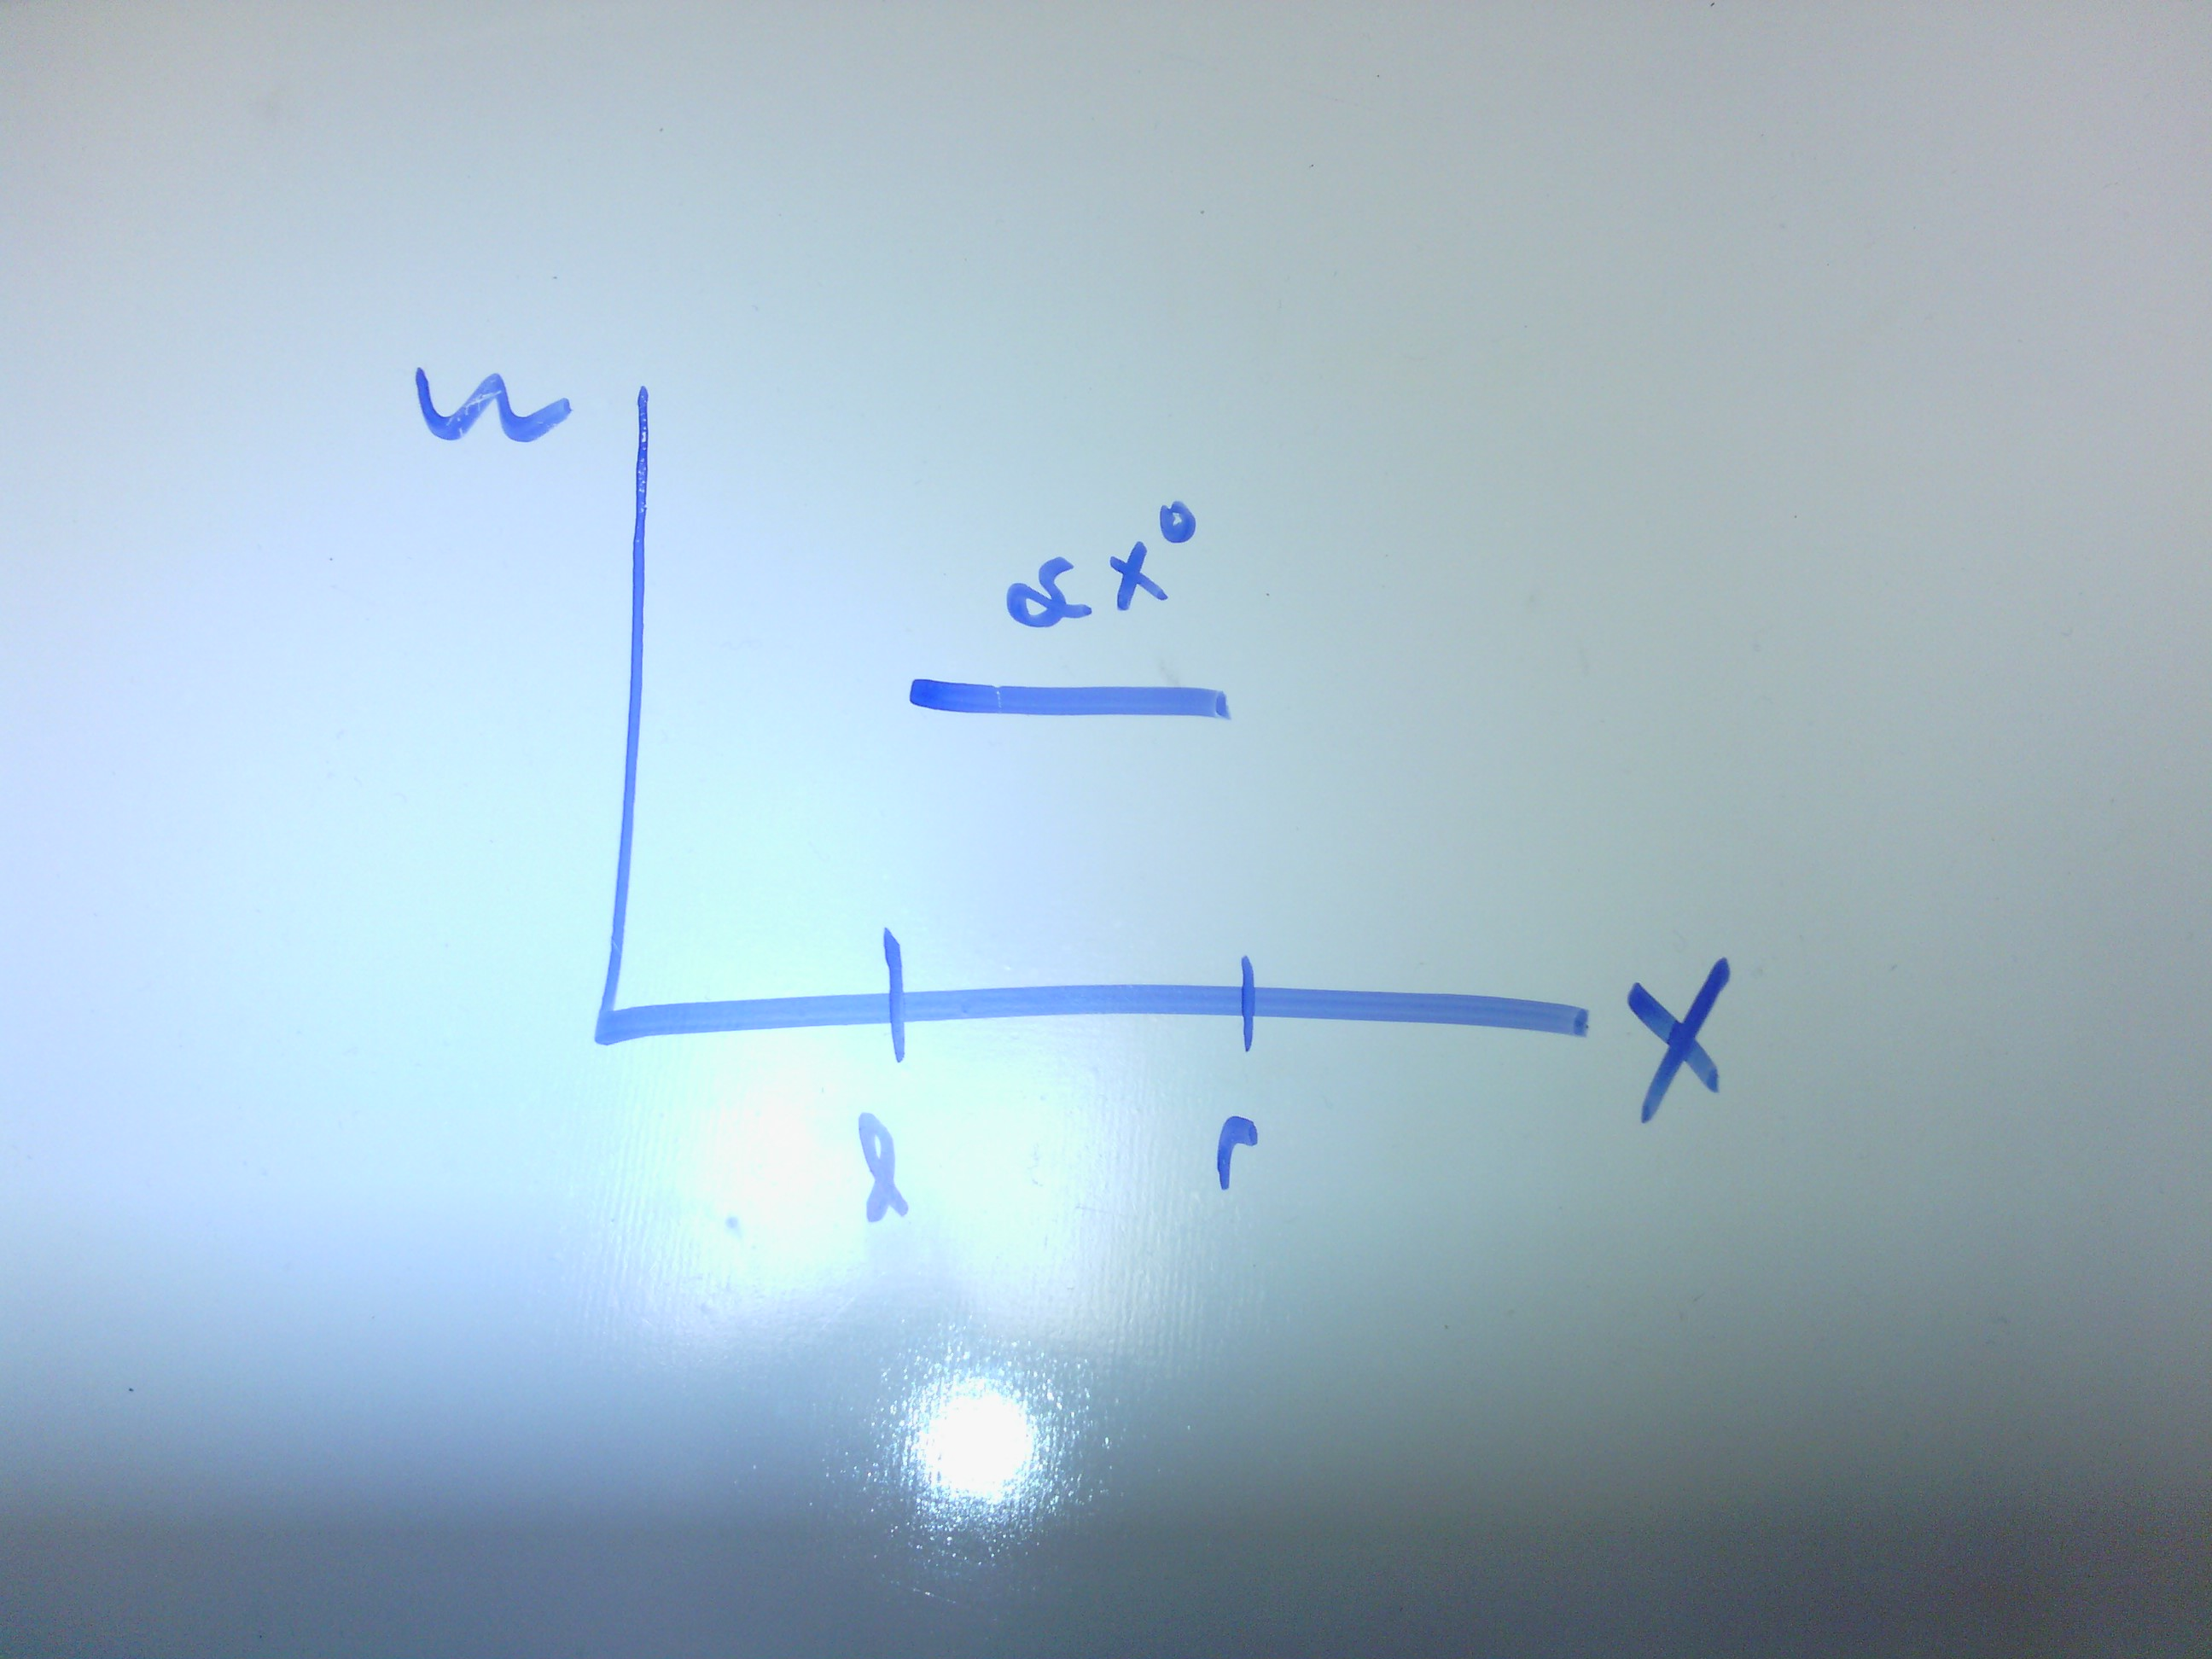
\includegraphics[scale=.1]{Jackson1-8-plates.jpg}
\caption{Energy density is zero outside the plates, and constant between them.}
\end{figure}

To get the total energy we would typically integrate the energy density over the volume. But since the energy density is constant in this case, we can simply multiply.
\begin{equation}
W=wAd
\end{equation}

Because the area, $A$, of the plates is infinite it should be clear that the total energy is also infinite. We can, however get a meaningful result by solving for energy per unit area.
\begin{equation}
\frac{W}{A}=wd=\frac{\sigma^2d}{2\epsilon_0}=\frac{\epsilon_0 V^2}{2d}
\end{equation}

\section{Concentric Spheres}
\begin{equation}
E=\frac{Q}{4\pi r^2\epsilon_0}
\end{equation}
We'll calculate the energy density in terms of charge, $Q$, and electric potential, $V$ as we did for he parallel plates. This time the charge-voltage relationship is $Q=\frac{4\pi\epsilon_0 V^2}{2r^4(b-a)^2}$.
\begin{equation}
w=\frac{\epsilon_0}{2}|\mathbf{E}|^2=\frac{Q^2}{32\pi^2r^4\epsilon_0}=\frac{a^2b^2\epsilon_0V^2}{2r^4(b-a)^2}\label{w-sphere}
\end{equation}

\begin{figure}[h]
\centering
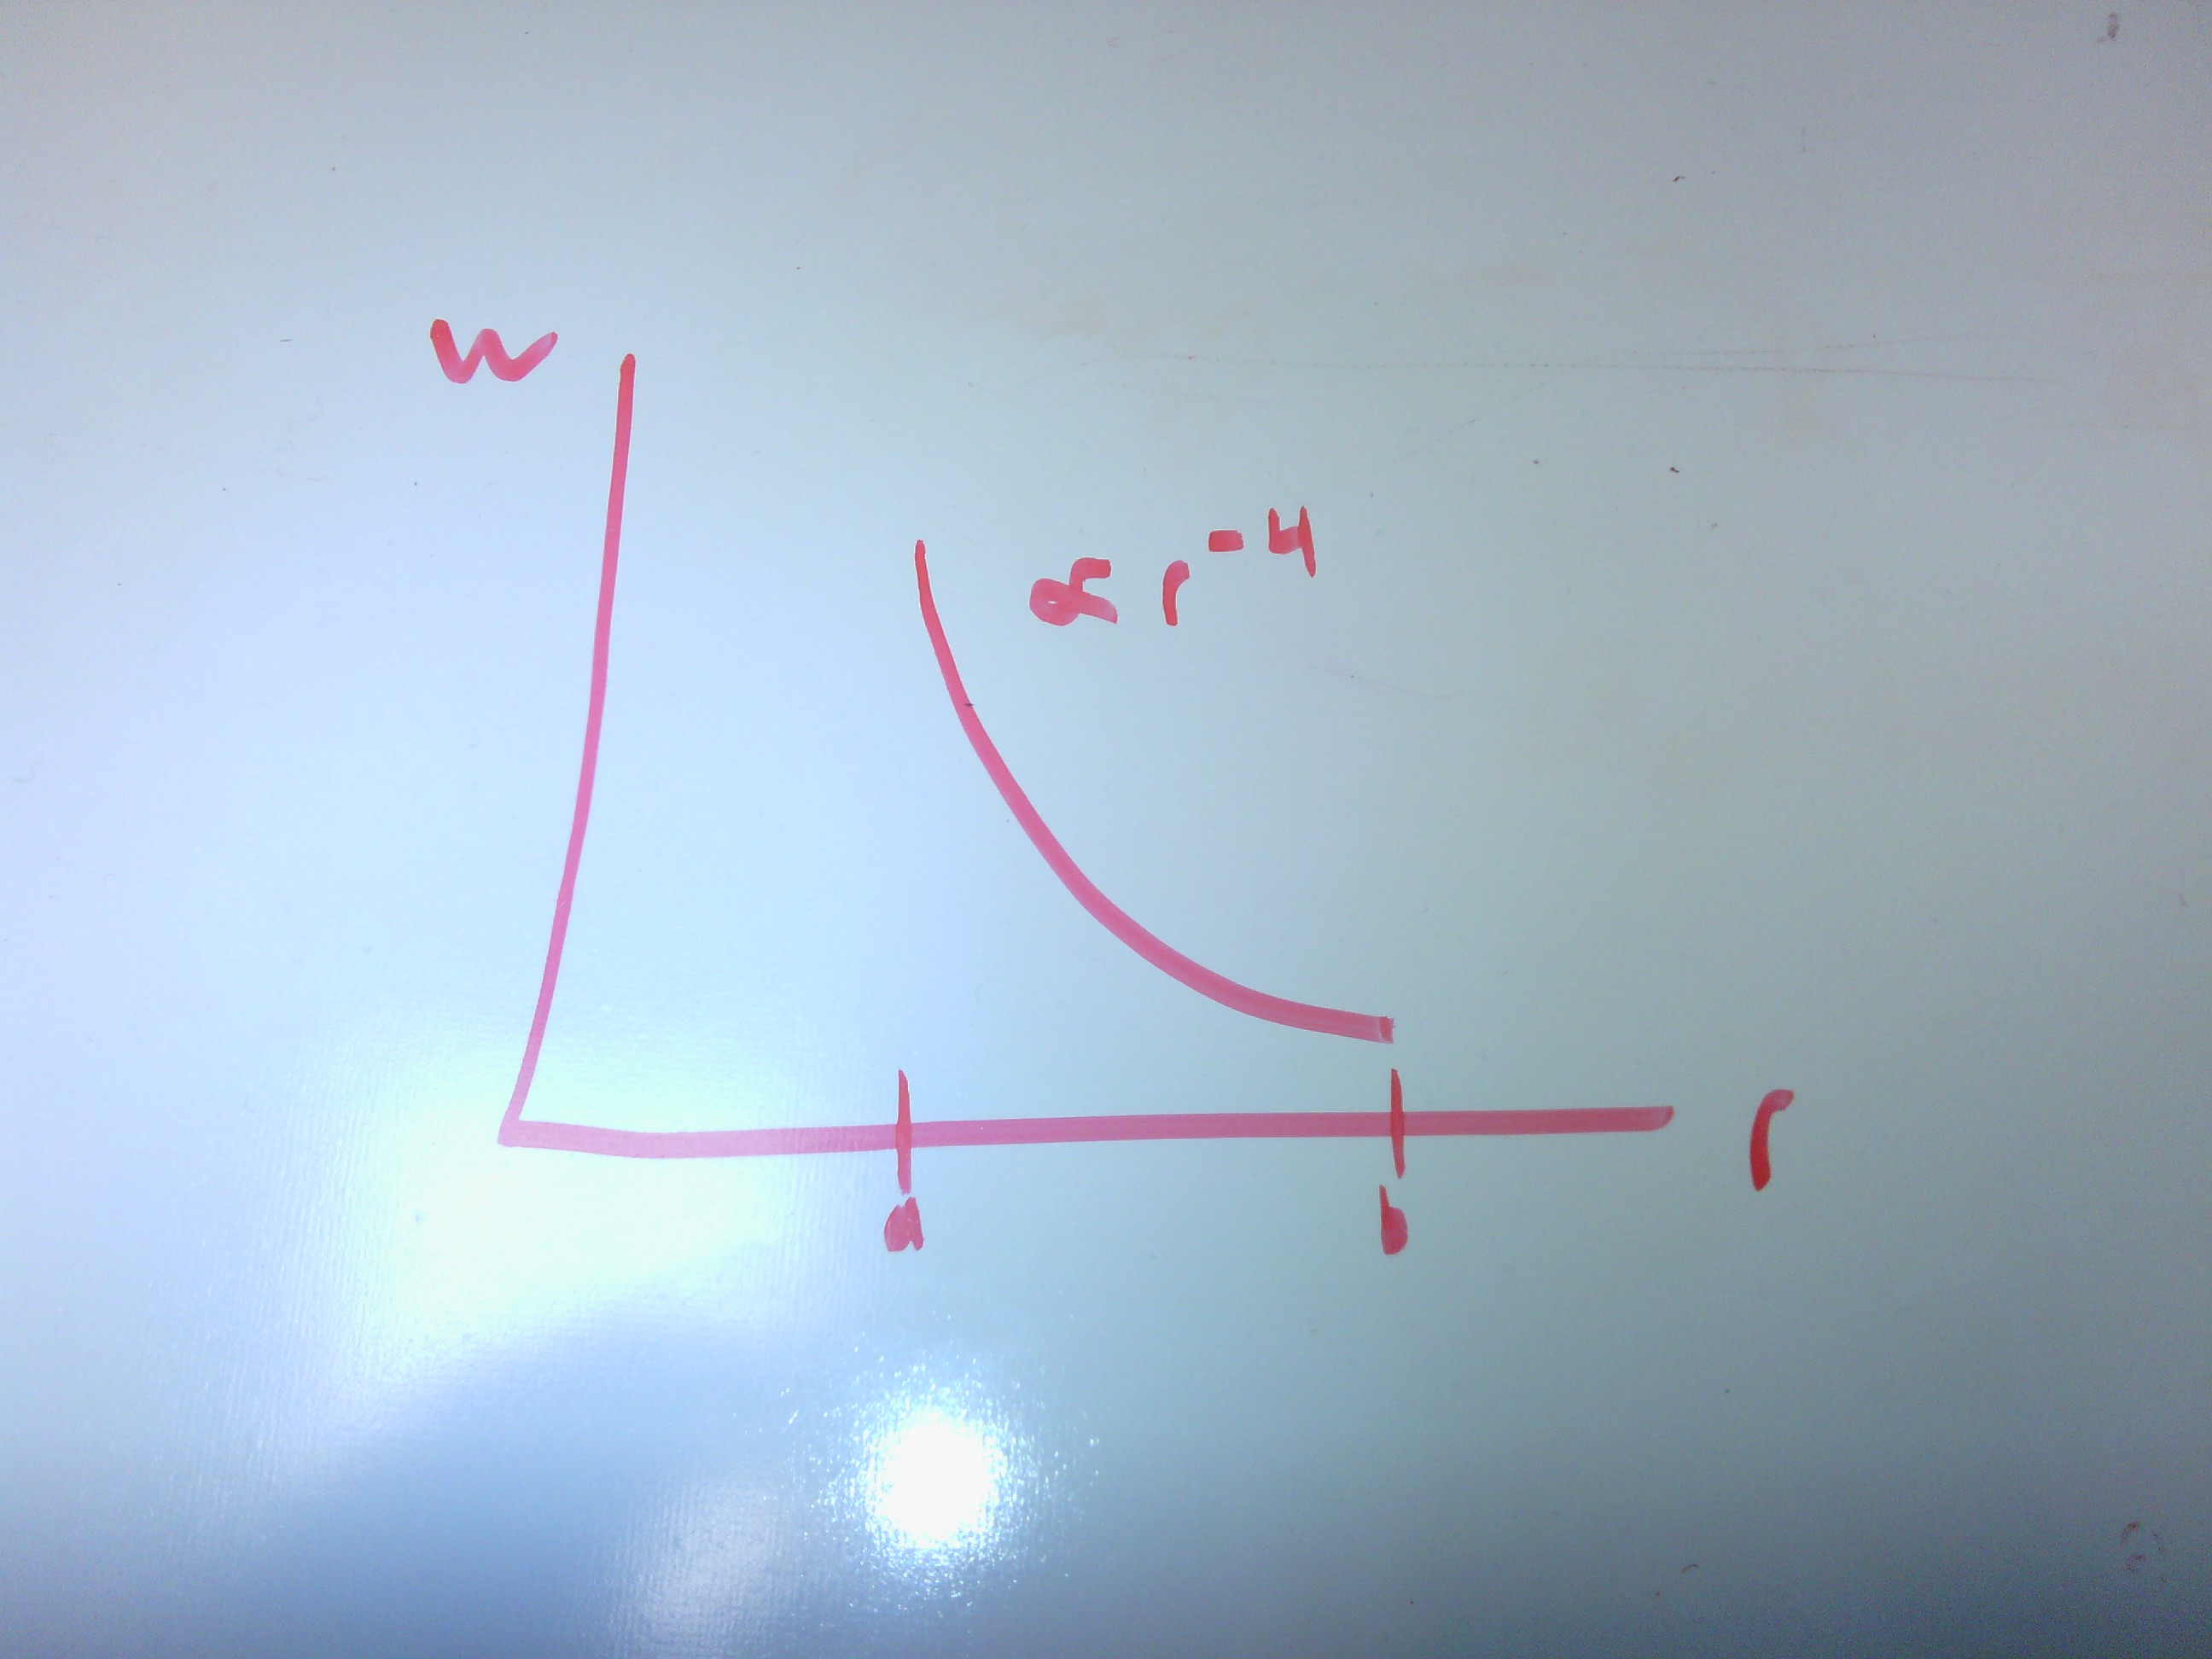
\includegraphics[scale=.1]{Jackson1-8-sphere.jpg}
\caption{Energy density is zero outside the spheres, and falls off as $1/r^4$ between them.}
\end{figure}

This time the energy density is not constant, so we will actually have to integrate.
\begin{equation}
W=\iiint w \,\mathrm{d}V
\end{equation}

Remembering that the angular integrals are relatively easy, $\iint_{sphere}\,\mathrm{d}\Omega=4\pi$, we can integrate equation \ref{w-sphere} as follows.
\begin{equation}
W=\frac{Q^2}{8\pi\epsilon_0}\int_a^b r^{-2}\,\mathrm{d}r
\end{equation}
\begin{equation}
W=\frac{Q^2}{8\pi\epsilon_0}\left[\frac{-1}{r}\right]_a^b
\end{equation}

Finally we arrive at the total energy (which is not infinite this time) in terms of charge and electric potential
\begin{equation}
W
=\frac{Q^2}{8\pi\epsilon_0}\left(\frac{1}{a}-\frac{1}{b}\right)
=\frac{2\pi\epsilon_0V^2}{\left(\frac{1}{a}-\frac{1}{b}\right)}
\end{equation}

\section{Concentric Cylinders}
\begin{equation}
E\frac{\lambda}{2\pi r\epsilon_0}
\end{equation}

We'll calculate the energy density as we did before noting that $\lambda=\frac{2\pi\epsilon_0V}{\ln(b/a)}$.
\begin{equation}\label{w-cylinder}
w
=\frac{\epsilon_0}{2}|\mathbf{E}|^2
=\frac{\lambda^2}{8\pi^2r^2\epsilon_0}
=\frac{\epsilon_0V^2}{2r^2\ln^2(b/a)}
\end{equation}

\begin{figure}[h]
\centering
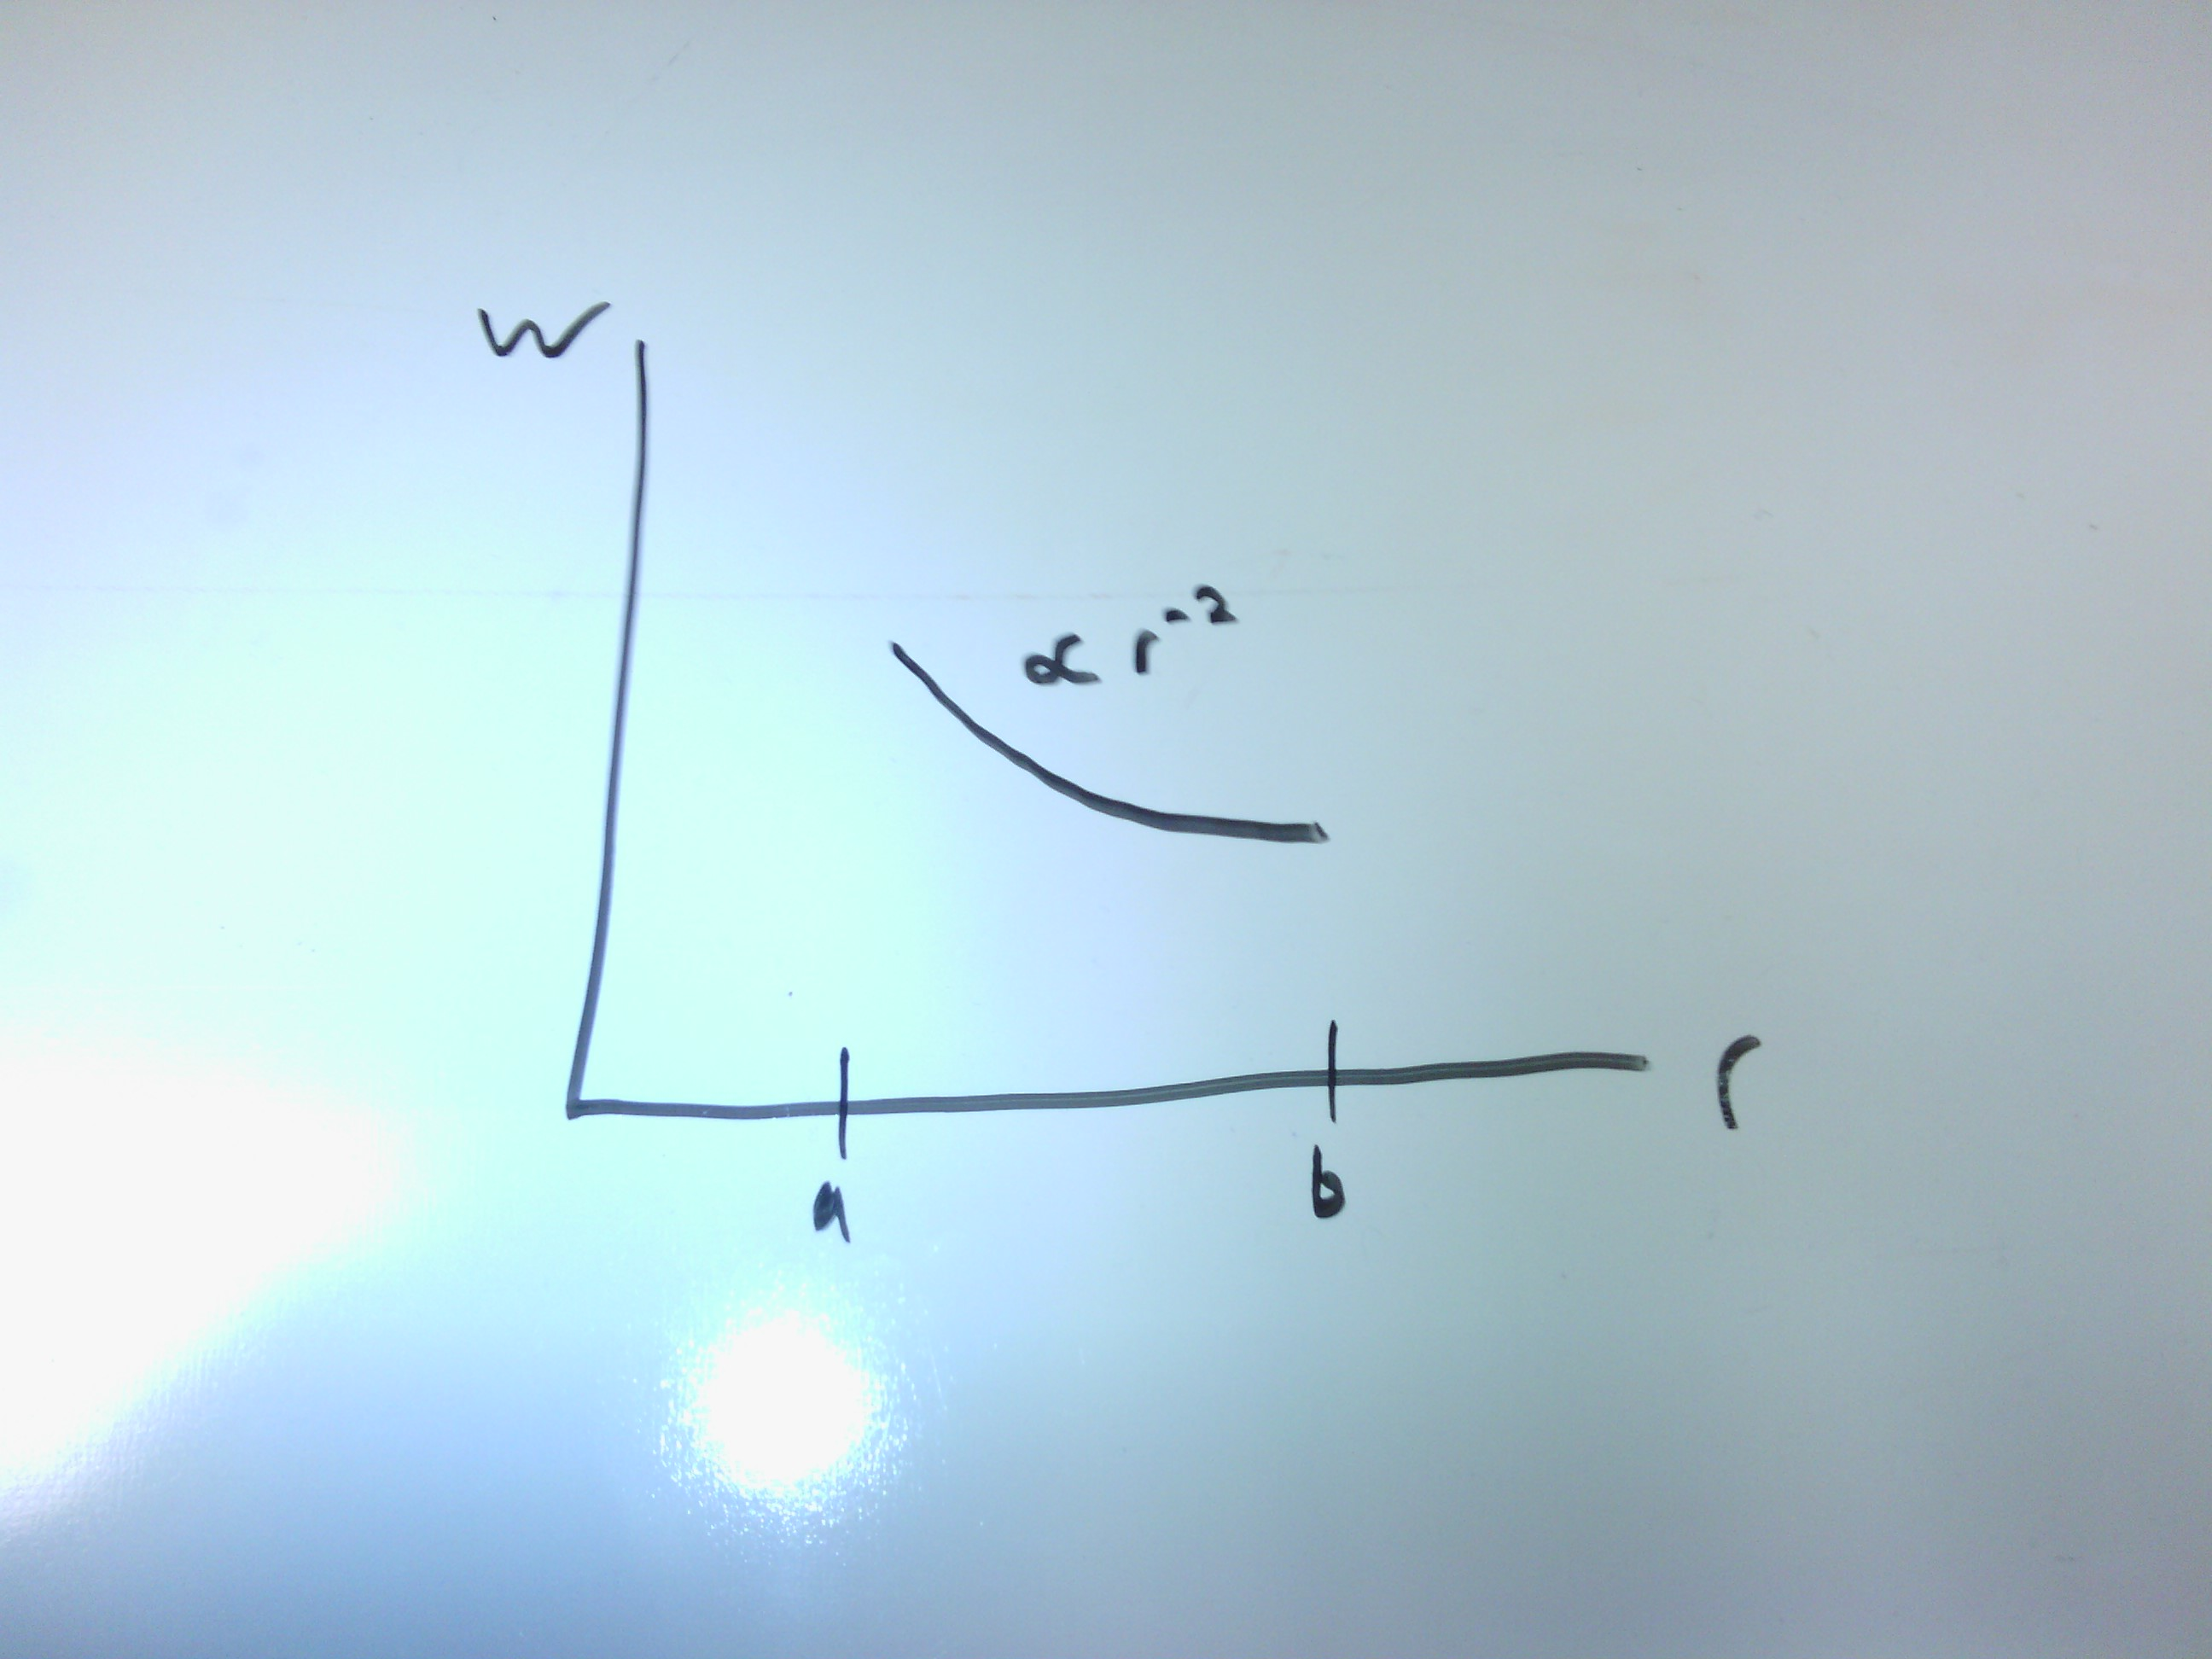
\includegraphics[scale=.1]{Jackson1-8-cylinder.jpg}
\caption{Energy density is zero outside the cylinders, and falls off as $1/r^2$ between them.}
\end{figure}

Like the case of parallel plates, the total energy is infinite. So we'll solve for Energy per length
\begin{equation}
\frac{W}{l}=\frac{\lambda^2}{4\pi\epsilon_0}\int_a^b \frac{1}{r}\,\mathrm{d}r
\end{equation}

The final result is then,
\begin{equation}
\frac{W}{l}
=\frac{\lambda^2}{4\pi\epsilon_0}\ln(b/a)
=\frac{\pi\lambda^2\epsilon_0 V^2}{\ln(b/a)}
\end{equation}

\end{document}